 % Este arquivo é uma adaptação do modelo LaTeX disponibilizado pelo UTUG (http://www.inf.ufrgs.br/utug/)
% Autor: Prof. Dr. Adriel M. Ziesemer Jr - IFRS Canoas
%
% Dica: Utilize o www.sharelatex.com para editar este documento. Utilize a opcão: Upload Zipped Project

\documentclass[openright]{ifrs} % utilize openright para iniciar capítulos no anverso
\usepackage[T1]{fontenc}        % pacote para conj. de caracteres correto
\usepackage[utf8]{inputenc}     % pacote para acentuaçao
\usepackage{graphicx}           % pacote para importar figuras
\usepackage{times}              % pacote para usar fonte Adobe Times
\usepackage{listings}
\usepackage{multirow}           % pacote para usagrupar células em tabelas
\usepackage{scalefnt}           % pacote para redimensionar fontes em tabelas
\usepackage{amsmath}
\usepackage{rotating}           % pacote para rotacionar figuras
\usepackage{color,graphicx}     % pacote coloração
\usepackage{hyperref}           %links
\bibliographystyle{abnt}

% ensine o latex a separar em sílabas as palavras que eventualmente ele não souber
\hyphenation{en-si-na-men-tos a-gra-de-ci-men-to de-se-nha-dos}

\author{Fraga}{Kael V. de O.}
%\author{Aluno2}{Nome do}

% edite o definicoes.sty se precisar alterar o nome do curso

\title{Pedal-to-Play: Um Sistema Web Gamificado para Monitoramento da Prática do Ciclismo}

%\advisor[Prof.~Dr.]{Pinto}{Rafael Coimbra}
\advisor[Prof.~Me.]{Pinto}{Rafael Coimbra}
%\coadvisor[Prof.~MSc.]{Co-orientador}{Nome do}

\location{Canoas}{RS}
%\date{julho}{2012} % se nao especificada, é utilizada a data atual

% palavras-chave (começar com letra maiúscula)
\keyword{Aplicativo de saúde e fitness}
\keyword{Geolocalização}
\keyword{Jogo pervasivo}
\keyword{Mobile}
\keyword{Web}

% nominata
\newcommand{\nominata}{
    %\MakeUppercase{\instituicao}\\
    %Reitora: Prof\textsuperscript{a}.~AAAAAA\\
    %Diretor do Instituto: Prof.~BBBBBBB\\
    %Coordenador do curso: Prof.~CCCCCCC\\
    %Bibliotecária-chefe: DDDDDDD
}

% inicio do documento
\begin{document}

% folha de rosto
\maketitle

% dedicatoria (opcional)
%\clearpage
%\begin{flushright}
%\mbox{}\vfill
%{\sffamily\itshape
%Dedico este trabalho à minha família.}
%\end{flushright}

% agradecimentos (opcional)
%\chapter*{Agradecimentos}
%Cita-los em ordem decrescente de importância.

% Resumo
%Arquivo contendo os Resumos
\begin{abstract}
O presente trabalho apresenta o desenvolvimento de um aplicativo "gamificado"\ com a pretensão de motivar seus usuários a praticarem a atividade de ciclismo. A popularização crescente dos \textit{smartphones} e \textit{tablets} trouxe consigo os aplicativos voltados para a saúde pessoal e condicionamento físico. Eles pretendem servir como ferramentas de auxílio ao usuário na prática de uma atividade física, em um cenário em que possuir uma rotina sedentária é comum e a prática constante de exercícios perde espaço. Um aplicativo que usa técnicas de gamificação tem a aspiração de motivar com mais eficiência um usuário que deseje persistir praticando uma atividade física, pois essas técnicas se apropriam dos elementos-chave que os jogos empregam para envolver o ser humano: a socialização, a competição, a fuga da realidade e o aprendizado. Ao longo deste trabalho são descritos os conceitos envolvidos para elaboração do projeto; trabalhos relacionados na mesma temática, os métodos para pesquisa, análise, projeto e desenvolvimento do \textit{software}; as tecnologias implementadas voltadas para Web, incluindo os \textit{frameworks} AngularJS e Bootstrap; o desenvolvimento para \textit{mobile} usando Cordova; o desenvolvimento do \textit{web service} REST com Slim; o uso de geolocalização para monitorar pedaladas do usuário; o módulo de avatar virtual; o módulo de desafios e recompensas e os \textit{softwares} terceiros agregados. Concluindo, são apresentados os resultados obtidos após a implementação da solução técnica, contendo \textit{print screens} das funcionalidades do \textit{software}, os testes envolvendo sessões reais de ciclismo e os objetivos cumpridos. 
\end{abstract}

\begin{englishabstract}
{Pedal-to-Play: A Gamified Web Application to Track Bicycle Rides}
{Health and Fitness application. Geolocation. Pervasive Game. Mobile}

This paper presents the development of a gamified application intended to motivate its users to practice cycling activity. The growing popularity of smartphones and tablets brought applications focused on health and  fitness. They plan to serve as tools in order to aid the user to practice a physical activity, in a scenario that maintaining a sedentary routine is common and practicing exercises loses ground. An application that implements gamification techniques aspires to motivate more efficiently an user that wishes to persist practicing a physical activity, because these techniques take ownership of the key elements that games employ to engage the human being: socializing, competition, escape from reality and learning. Throughout this paper are described the concepts involved in this project development; works related to the same theme, the methods of research, analysis, project design and development of software; the implemented technologies for Web, including the frameworks AngularJS and Bootstrap; development for mobile devices using Cordova; REST web service development with Slim; the use of geolocation to track user rides; the virtual avatar module; the challenges and rewards module and third party softwares aggregated. After the implementation of the technical solution, the results obtained are presented, containing print screens of software features, tests involving real rides and achieved goals.
\end{englishabstract}

% lista de abreviações
% Arquivo contendo a lista de abreviaturas e siglas
\begin{listofabbrv}{SPMD}
        \item[AJAX] Asynchronous Javascript and XML 
        \item[API] Application Programming Interface 
        \item[ASP] Active Server Pages
        \item[CORS] Cross Origin Resource Sharing
        \item[CSS] Cascading Style Sheets
        \item[DAO] Data access object
        \item[GPS] Global Positioning System 
        \item[GUI] Graphical User Interface
        \item[HTML] Hyper Text Markup Language
        \item[HTTP] Hypertext Transfer Protocol
        \item[IE] Internet Explorer
        \item[Java EE] Java Enterprise Edition
        \item[JS] JavaScript
        \item[JSON] JavaScript Object Notation
        \item[JSP] JavaServer Pages 
        \item[MVC] Model-View-Controller
        \item[PHP] PHP: Hypertext Preprocessor
        \item[REST] Representational State Transfer
        \item[SOAP] Simple Object Access Protocol
        \item[SGDB] Sistema de Gerenciamento de Banco de Dados
        \item[SSH] Secure Shell
        \item[SVG] Scalable Vector Graphics
        \item[UML] Unified Modeling Language
        \item[URL] Uniform Resource Locator
        \item[W3C] World Wide Web Consortium
        \item[WLAN] Wireline Local Area Network
        \item[XML] eXtensible Markup Language
\end{listofabbrv}

% lista de figuras
\listoffigures

% lista de tabelas
\listoftables

% lista de símbolos (opcional)
%\begin{listofsymbols}{$\alpha\beta\pi\omega$}
%       \item[$\sum{\frac{a}{b}}$] Somatório do produtório
%       \item[$\alpha\beta\pi\omega$] Fator de inconstância do resultado
%\end{listofsymbols}

% sumário
\tableofcontents

% Introdução
%Arquivo contendo o capítulo Introdução
\chapter{Introdução} \label{cap:introducao}
Atualmente, \textit{smarthphones} e aplicativos para acompanhamento de atividades físicas e saúde pessoal estão bem popularizados, eles buscam motivar seus usuários a continuar praticando exercícios e dedicando tempo de suas vidas para saúde. Todavia, esses resultados não são instantâneos e nesta época de bombardeio de informações, o \textit{feedback} demorado da prática de um exercício vem a desmotivar os iniciantes, entre outros fatores, como tais: a exaustiva rotina diária e a falta de acompanhamento para a atividade. \par 

Nestes pontos fracos que os aplicativos modernos de acompanhamento de atividades físicas atacam, se tornando companheiros de bolso para qualquer um que deseje praticar um esporte, mesmo que por lazer. Eles proporcionam a socialização através das redes sociais, \textit{feedback} instantâneo através dos dados coletados via funcionalidades dos \textit{smarthphones} e competição por melhores desempenhos entre os usuários do mesmo aplicativo. \par

O modo de vida contemporâneo é outro fator que não favorece a prática de exercícios físicos, pois a maior parte do dia da população é ocupada por trabalho ou estudo, senão ambos. Entre estes dois também há o quesito trânsito. O tempo livre restante é aproveitado para descanso ou socialização com família ou com amigos. Aqueles que praticam esportes por \textit{hobbie} encontram, ao passar o tempo, cada vez mais obstáculos para praticá-los: seja por falta de tempo, por problemas econômicos e financeiros ou por simplesmente não sentir prazer na atividade praticada \cite{butcher2002, liz2013}. \par

Vivendo neste cenário, onde a prática de uma atividade física não se torna hábito em nossas vidas (embora seja necessário para manter nosso corpo e mente saudáveis) surge o questionamento, de que maneira um \textit{software} poderia motivar os usuários a persistirem na prática de um exercício, mais especificamente, a atividade de ciclismo? \par

Assim, a pesquisa fruto desse projeto pretende desenvolver um \textit{software} multiplataforma (\textit{mobile} e \textit{desktop}) que use as tecnologias de desenvolvimento \textit{Web} e aplique conceitos de gamificação no formato de um jogo pervasivo, o qual será denominado Pedal-to-Play. \par

Entre as funcionalidades do Pedal-to-Play, propõe-se a captura e processamento de determinados dados durante as seções de ciclismo do usuário, com o fim de mensurar o desempenho dele na atividade, recompensando-o com pontos e \textit{badges} (troféus virtuais e indicadores de realização de tarefas) de acordo com os resultados alcançados. Pretende-se possibilitar o compartilhamento das recompensas em redes sociais. O \textit{software} também possuirá um sistema de \textit{avatar} virtual customizável, o qual ilustrará o perfil do usuário, contendo informações sobre a evolução do mesmo na atividade de ciclismo.

\section{Motivação}
Diferente dos \textit{softwares} que somente coletam os dados do usuário e os exibem de forma gráfica, um sistema que implementa técnicas de gamificação em seu desenvolvimento propõe alternativas para a superação de fatores desmotivadores na prática de uma atividade. As técnicas de gamificação  trabalham estimulando os principais fatores motivadores para o ser humano: competição, aprendizado, fuga da realidade e interação social \cite{vianna2013}. Assim, o Pedal-to-Play proporá desafios ao usuário e o mesmo será recompensado pela participação neles. Buscando concomitantemente conciliar o entretenimento na atividade exercida pelo usuário e permitindo a socialização com outros ciclistas que também façam uso do \textit{software}. \par

A atividade de ciclismo foi escolhida como foco do trabalho pelos benefícios a saúde do praticante, ao meio ambiente e a mobilidade urbana. \citet{rojasrueda2011} constatou que o aumento de adeptos à bicicleta como meio de transporte na cidade de Barcelona ocasionou na diminuição de acidentes no trânsito e a diminuição de gás carbônico no ambiente.

\section{Objetivo}
Este trabalho possui os seguintes objetivos:

\subsection{Objetivo Geral}
Desenvolver um \textit{software} com a pretensão de motivar o usuário a persistir praticando a atividade de ciclismo. 

\subsection{Objetivos Específicos}
\begin{itemize}
\item Identificar quais dados devem ser analisados e como computá-los para mensurar o desempenho do ciclista;
\item Identificar e selecionar quais \textit{frameworks} e linguagens de programação adequados para o desenvolvimento do \textit{software};
\item Desenvolver uma interface homem-computador responsiva e multiplataforma;
\item Desenvolver um mecanismo dentro da aplicação para propor desafios ao usuário e recompensá-lo pela participação nestes;
\item Permitir ao usuário compartilhar seus dados contidos no \textit{software} em redes sociais;
\item Analisar e aplicar técnicas de gamificação para o desenvolvimento do \textit{software}.
\end{itemize}

\section{Organização do Texto}
Este documento está divido em três capítulos. O capítulo \ref{cap:metodologia} versa os métodos que serão utilizados para a elaboração da pesquisa e o desenvolvimento do \textit{software}, assim como descreve as etapas do trabalho e as funcionalidades que pretende-se implementar. O capítulo \ref{cap:cronograma} conterá uma tabela contendo as tarefas fundamentais deste trabalho e em qual mês cada uma delas será efetuada.
O cronograma abrange quatro meses do segundo semestre de 2015.



% Revisao Bibliográfica
%%Arquivo contendo o capítulo Revisão Bibliográfica
\chapter{Revisão Bibliográfica} \label{cap:revbib}
Esse capítulo tem como objetivo descrever os principais conceitos apresentados para o desenvolvimento do \textit{software} proposto. Os conceitos envolvidos são: jogo pervasivo; gamificação; desenvolvimento multiplataforma; aplicativos de saúde e \textit{fitness}; avatares virtuais e geolocalização.

\section{Jogos Pervasivos}
Um jogo pervasivo é um tipo de jogo digital, no qual ao menos uma interação do usuário com o sistema transcorre no universo físico. Eles integram os aspectos físicos e sociais do mundo real em jogos digitais, estendendo a interação do jogador com o jogo, pois em ambientes virtuais a interface com o usuário está limitada ao uso dos periféricos do computador. Os recentes dispositivos celulares (\textit{smartphones}) e a popularização de tecnologias de rede sem fio 
(tais como, \textit{WiFi\footnote{WiFi é o termo popular para redes sem fio ethernet padrão  WLANs (Wireline Local Area Networks) \cite{lehr2003}.} e 3G\footnote{3G refere-se a terceira geração de serviços de dados móveis, fornecido por operadoras provedoras de redes móveis \cite{lehr2003}.}}) facilitam a extensão das interfaces homem-computador. \cite{magerkurth2005, vianna2013}. Um exemplo de jogo pervasivo é o Human Pacman. \par

\begin{figure}[h]
    \caption[Processo de coleta de um item no Human Pacman]{Processo de coleta de um item no Human Pacman \cite{cheok2003}.}
    \centerline{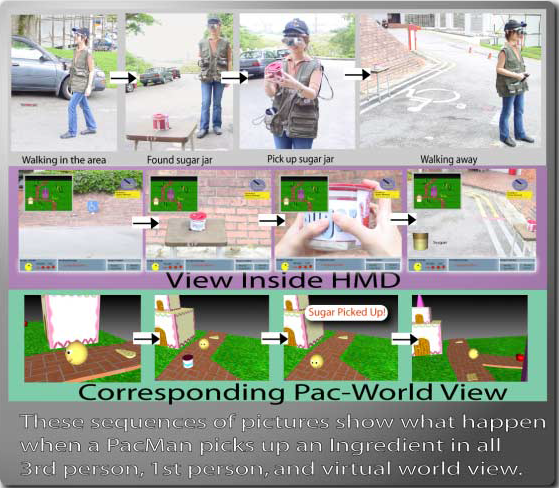
\includegraphics[width=20em]{figuras/humanpacman.png}}
    \label{fig:humanpacman}
\end{figure}

No Human Pacman, os jogadores interpretam o papel dos personagens do jogo Pac-Man no mundo real, enquanto vestem-se com trajes customizados integrados a dispositivos eletrônicos. Esses trajes permitem interação entre os jogadores via WiFi e interação com o sistema que insere elementos virtuais no mundo físico, através de técnicas de realidade aumentada, como ilustrado na figura \ref{fig:humanpacman} \cite{cheok2003}. 

\section{Gamificação}
A gamificação (do original em inglês \textit{gamification}) consiste na aplicação de mecanismos de jogos com o intuito de resolver problemas práticos ou motivar um público específico a realizar certas atividades em contextos fora de jogos. Alguns exemplos de aplicação de gamificação tem como objetivo: agilizar processos de aprendizagem ou treinamento; tornar mais agradáveis tarefas consideradas tediosas ou repetitivas; motivar usuários a reforçar a condição física e emocional e até usar jogos em forma de propagandas de produtos e serviços. O Duolingo\footnote{\url{https://www.duolingo.com/}} é um exemplo de \textit{software} "gamificado" para agilizar processos de aprendizagem de uma língua estrangeira e o SuperBetter\footnote{\url{https://www.superbetter.com/}}, para incentivar o usuário a reforçar o condicionamento físico. \cite{vianna2013, zichermann2011}.

\section{Desenvolvimento Multiplataforma}
Com a intenção de garantir que o \textit{software} possua portabilidade para plataformas \textit{mobile} e \textit{desktop} se fará uso do desenvolvimento \textit{Web}. Segundo \citet{lopes2013}, o desenvolvimento \textit{Web} é democrático, aberto e acessível, pois praticamente, todo dispositivos possui um navegador (\textit{web browser}). Uma aplicação \textit{Web} garante acesso a um número maior de usuários do que uma aplicação nativa para um determinado dispositivo. Lopes também salienta que é cada vez mais comum usar as linguagens fundamentais da \textit{Web} para desenvolver aplicativos \textit{mobile}. A subseção seguinte versará sobre as tecnologias fundamentais do desenvolvimento \textit{Web}.

\subsection{Lado do Cliente}
As tecnologias fundamentais usadas em sistemas \textit{Web}, no lado do cliente, são o HTML (\textit{Hyper Text Markup Language}), o CSS (\textit{Cascading Style Sheets}) e o JavaScript (JS). \par

HTML5 é a versão atual do HTML, linguagem de marcação para escrever a estrutura principal de páginas \textit{Web}. HTML fornece instruções aos \textit{web browsers} (exemplos: Chrome, IE, Firefox) sobre o que exibir em uma página. Cada conteúdo é representado por um conjunto de elementos pré-definidos chamados \textit{tags} \cite{html5}. \par 

CSS é a linguagem usada para definir o estilo e o \textit{layout} do conteúdo de uma página HTML. Ela também permite ajustar o \textit{layout} das aplicações para qualquer tamanho de tela, inclusive o \textit{mobile}. Esta característica é importante para o \textit{software} desde trabalho, o qual pretende ser multiplataforma. A versão atual do CSS é o CSS3 \cite{css3}. \par
 
JS é uma linguagem de programação interpretada e orientada a objetos, usada para manipular o comportamento de páginas HTML. Possui recursos para alterar o conteúdo das páginas, o estilo delas e validar entradas do usuário. \cite{javascript}. \par

No desenvolvimento do lado do cliente também podem ser empregados \textit{frameworks} e bibliotecas. Estes se propõem a facilitar o uso das linguagens listadas anteriormente, assegurar questões de compatibilidade entre navegadores, assegurar questões de segurança e confiabilidade e de portabilidade para diferentes dispositivos. \par

Os seguintes \textit{frameworks} serão investigados para o possível uso no desenvolvimento do \textit{software} deste trabalho: Bootstrap\footnote{\url{http://getbootstrap.com/}}, para desenvolvimento de páginas \textit{Web} responsivas e adaptáveis para dispositivos com tamanhos diversos; AngularJS\footnote{\url{https://angularjs.org/}}, usado para tornar páginas HTML estáticas em páginas dinâmicas, estendendo o vocabulário do HTML; e jQuery\footnote{\url{https://jquery.com/}}, usado para facilitar e estender o JS. \par
 
A plataforma Cordova\footnote{\url{https://cordova.apache.org/}}, para conversão de sistemas \textit{Web} em aplicações nativas \textit{mobile}, também será investigada. Ela permite atribuir ao \textit{software} acesso aos recursos de \textit{hardware} dos dispositivos \textit{mobile}.

\subsection{Lado do Servidor} \label{sec:server}
Atualmente o pódio das tecnologias para o desenvolvimento \textit{Web} do lado do Servidor está ocupado pelo PHP, em primeiro lugar; ASP.NET em segundo e o Java, em terceiro \cite{w3techs2015}. \par

Java \textit{Web} consiste na implementação das APIs de Servlets e JavaServer Pages (JSP). Servlet é a tecnologia usada pelo Java para geração de páginas HTML dinâmicas, são classes Java com HTML embutido. Páginas JSP consistem no inverso, são estruturadas como páginas HTML com código Java embutido. Servlets e JSP podem ser desenvolvidos na plataforma Java Enterprise Edition (Java EE). A Java EE consiste em um conjunto de especificações para várias APIs de desenvolvimento Java para \textit{Web} \cite{basham2008}. Os pontos fortes do Java \textit{Web} estão na portabilidade para diferentes plataformas de \textit{hardware}, banco de dados e servidores e a grande quantidade de \textit{frameworks} existentes, tais como Primefaces\footnote{\url{http://www.primefaces.org/}} e Spring\footnote{\url{http://spring.io/}}. \par

ASP.NET é uma tecnologia da Microsoft, parte do .NET \textit{Framework} para desenvolvimento de aplicações \textit{Web}. O desenvolvimento com ASP.NET pode ser feito com qualquer linguagem compatível com o .NET. Algumas das vantagens desta tecnologia envolvem a separação clara entre a interface do usuário e a lógica de programação; a familiaridade com o desenvolvimento \textit{desktop}; a ferramenta de desenvolvimento Visual Studio, com diversos recursos para facilitar o trabalho do desenvolvedor e a integração com todos os recursos do \textit{framework} .NET \cite{imar2014}. As desvantagens do ASP.NET são: sua limitação ao sistema operacional Windows e a licença de uso do Visual Studio não ser gratuita. \par

PHP é uma linguagem de programação presente em 10 milhões de sites no mundo inteiro. O PHP adiciona dinamismo às páginas estáticas e automatiza tarefas, diminuindo mão-de-obra. Possui portabilidade para várias plataformas \textit{desktop} (exemplos: Linux, Unix e Windows); possui código aberto e licença de uso gratuita; suporta vários bancos de dados (entre eles: MySQL, Oracle e PostgreSQL). Sua versão mais recente é o PHP 5 \cite{niederauer2004, welling2003}. \par

Outros pontos fortes do PHP envolvem sua alta performance (um único servidor pode lidar com milhões de acessos por dia); bibliotecas nativas para várias tarefas comuns na \textit{Web} (funções para gerenciamento de imagens, conexão com \textit{web services}, interpretação de XML, envio de \textit{email}, gerenciamento de \textit{cookies} e geração de documentos PDF); fácil aprendizado (a sintaxe de PHP é baseada em outras linguagens, entre elas, C e Perl); suporte ao desenvolvimento orientado a objetos e disponibilidade de suporte técnico \cite{welling2003}. \par

Pretende-se usar a linguagem PHP para desenvolvimento do lado do servidor, pois comparado com as outras duas principais linguagens (ASP.NET e Java) o PHP se destaca por sua licença gratuita, portabilidade e suporte nativo (sem \textit{frameworks}) a funcionalidades que serão essenciais no software deste trabalho, tais como: gerenciamento de imagens, interpretação de arquivos JSON e acesso a banco de dados. \par

No quesito sistemas de gerenciamento de bando de dados (SGDB), os três mais usados atualmente segundo o \textit{site} da DB-Engines são o Oracle em primeiro lugar, o MySQL em segundo e o Microsoft SQL Server em terceiro. O MySQL possui licença de uso \textit{open source} e versão gratuita sem restrições, enquanto o Oracle e o Microsoft SQL Server são \textit{softwares} com licença de uso comercial, por estes motivos pretende-se fazer uso dele. \par

\section{Aplicativos de Saúde e \textit{Fitness}}
Aplicativos de Saúde e \textit{Fitness} são \textit{softwares} desenvolvidos para dispositivos \textit{mobile} com o objetivo de estimular o usuário a praticar atividades benéficas à saúde e ao bem-estar \cite{bonome2012}. Alguns exemplos dessa categoria de aplicativos são o Strava\footnote{\url{https://www.strava.com/}} e o  Runtastic\footnote{\url{https://www.runtastic.com/}}. \par

\section{Avatares Virtuais}
Avatares são corpos virtuais criados para representar a identidade e ações de um usuário em um mundo virtual. Eles são usados como ferramentas de comunicação e para representar visualmente os usuários. Uma das principais características dos avatares é a sua customização, orientada pelo desejo de quem o cria \cite{ducheneaut2009}. Um exemplo de aplicativo específico para criação de avatares e utilização destes como ferramente de socialização entre os usuários é o \textit{BuddyPoke}, ver figura \ref{fig:avatar}. \par

\begin{figure}[hb]
    \caption{Exemplo de avatar criado no aplicativo BuddyPoke.}
    \centerline{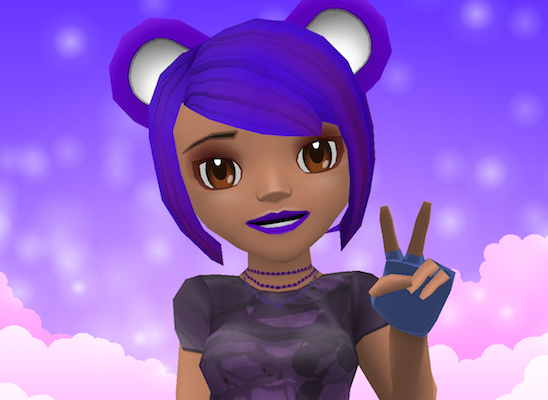
\includegraphics[width=17em]{figuras/avatar.png}}
    \label{fig:avatar}
\end{figure}
\centerline{Fonte: Página oficial do BuddyPoke na \textit{Web}\footnote{Disponível em: <\url{http://www.buddypoke.com/}>. Acesso em jun. 2015.}}

\section{Geolocalização}
Geolocalização é o termo usado para descrever o posicionamento geográfico de um objeto no planeta, a partir de seus valores de latitude e longitude \cite{aires2014}. Essas coordenadas são obtidas utilizando \textit{Global Positioning System} (GPS), um sistema desenvolvido e mantido pelas Forças Aéreas dos Estados Unidos. Este sistema consiste em três segmentos: o espacial, composto por 24 satélites operantes em órbita e transmitindo sinais de radio; o controle, o qual consiste nas estações de controle que mantêm os satélites funcionando adequadamente; e o segmento do usuário, o qual compreende os aparelhos receptores dos sinais vindos dos satélites \cite{gpsgov}. O funcionamento do GPS é ilustrado na figura \ref{fig:gps}. \par

\begin{figure}[h]
    \caption[Funcionamento do GPS]{Funcionamento do GPS \cite{cesani2013}.}
    \centerline{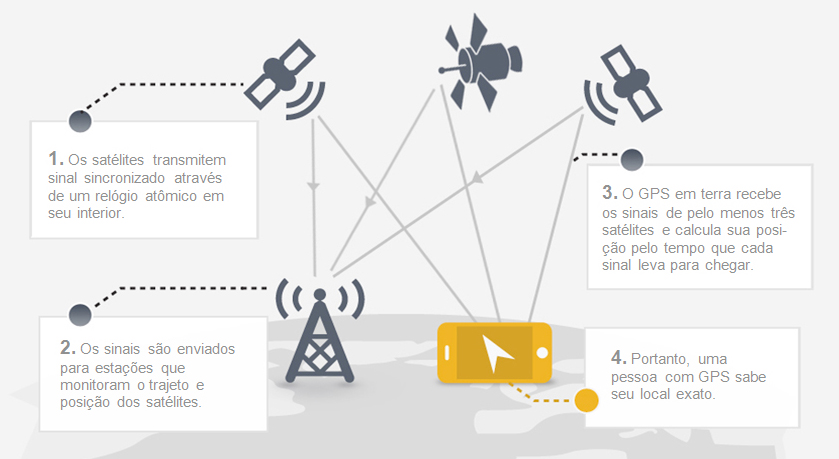
\includegraphics[width=30em]{figuras/gps.png}}
    \label{fig:gps}
\end{figure}

No entanto, o uso de GPS tem suas limitações. Segundo \citet{sukaphat2013}, os sinais de GPS possuem um alcance limitado e uma capacidade baixa de atravessar barreiras. Estas características impedem o funcionamento adequado desta tecnologia em ambientes fechados. \par

%\section{Conclusões}
%Reunir as ideias principais abordadas no capítulo.

% Estado da Arte
%%Arquivo contendo a sessão Estado da Arte
\chapter{Estado da Arte} \label{cap:estadoarte}
Nesta seção serão descritos alguns trabalhos relacionados com a temática e conceitos do Pedal-to-Play. Eles serão divididos em dois grupos: aplicativos comerciais e trabalhos científicos.

\section{Aplicativos comerciais}
Entre os aplicativos comerciais mais populares atualmente na categoria de Saúde e \textit{Fitness}, com a atividade de ciclismo como um dos focos, estão o Strava e o Runtastic Road Bike. Ambos utilizam funções do geolocalização para traçar rotas, guardar trajetos do usuário e calcular valores de velocidade, altitude e distância percorrida, com a intenção de gerar relatórios sobre o desempenho do usuário em corridas ou pedaladas. As Figuras \ref{fig:strava} e \ref{fig:Runtastic} são \textit{print screens}, respectivamente, dos aplicativos Strava e Runtastic Road Bike.\par 

\begin{figure}[h]
\centering
\begin{minipage}{.5\textwidth}
  \centering
  \captionof{figure}{Rastreamento de pedalada\\do Strava.}
  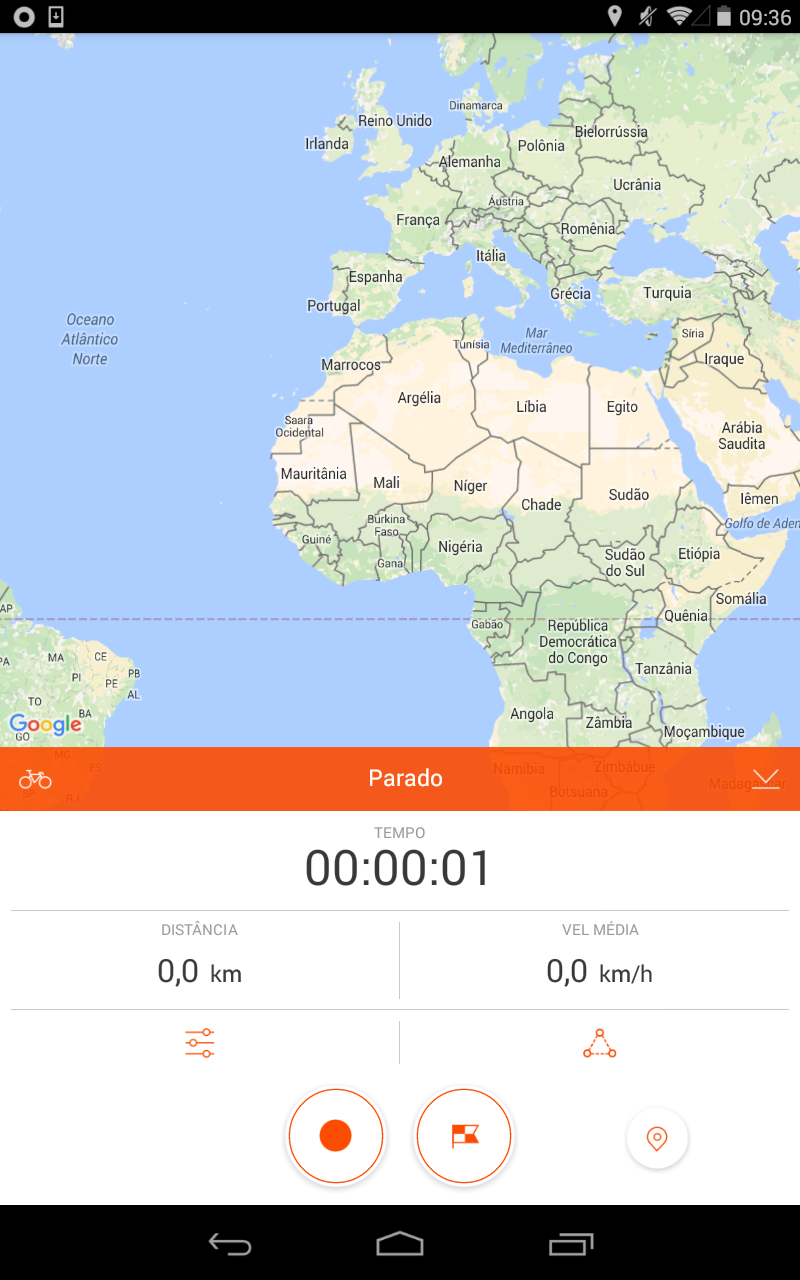
\includegraphics[width=.8\linewidth]{figuras/strava.png}
  \label{fig:strava}
  \newline
\end{minipage}%
\begin{minipage}{.5\textwidth}
  \centering
  \captionof{figure}{Histórico de atividades\\do Runtastic Road Bike.}
  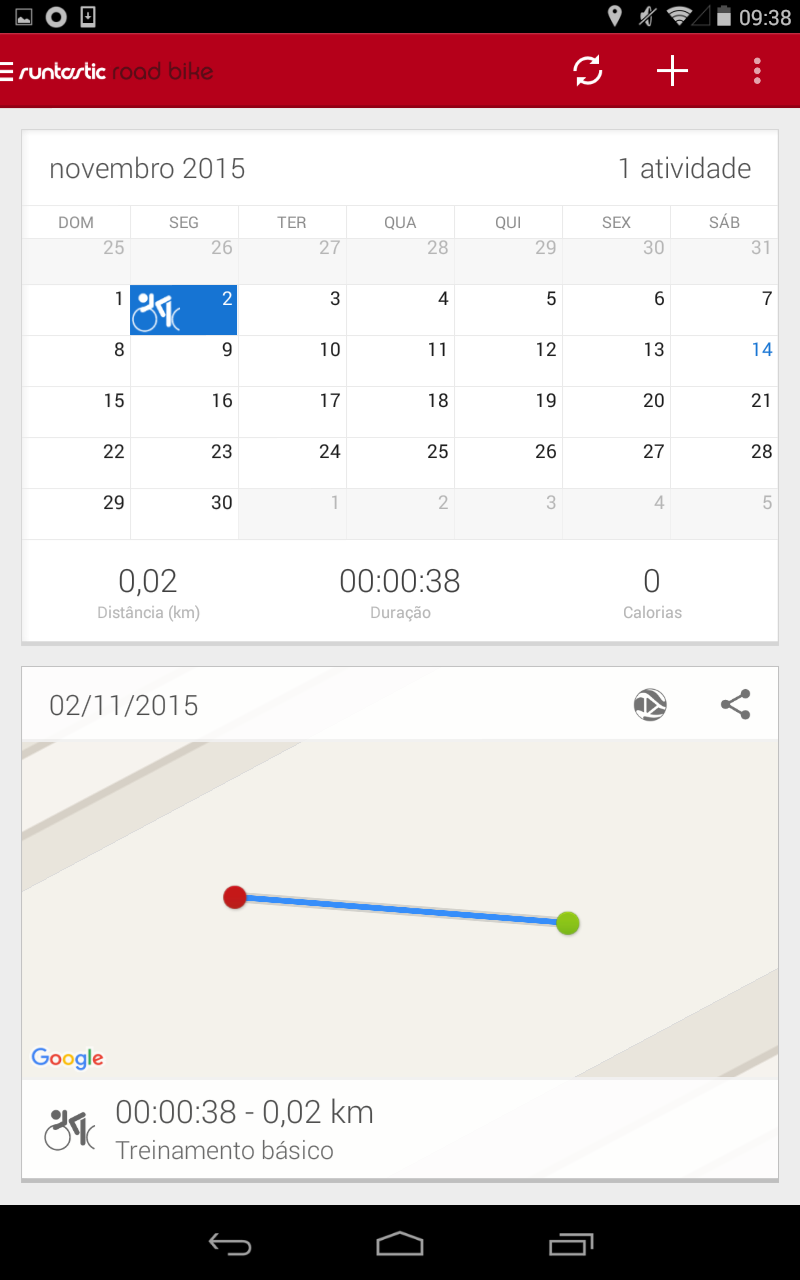
\includegraphics[width=.8\linewidth]{figuras/Runtastic.png}
  \label{fig:Runtastic}
  \newline
\end{minipage}
\centerline{Fonte: \textit{print screens} das aplicações Strava e Runtastic Road Bike, respectivamente.}
\end{figure}

O Strava, em particular, utiliza alguns conceitos de gamificação, tais como: sistema de desafios e recompensas (baseadas em prêmios, \textit{ranking} e \textit{badges}); criação de metas e socialização entre usuários. \par 

Estes aplicativos também possibilitam integração com redes sociais e compartilhamento de dados entre os usuário. Assim como o interfaceamento com outros dispositivos eletrônicos para monitoramento de atividades, tal como o Garmin\footnote{\url{http://www.garmin.com/}} (Figura \ref{fig:garmin}). \par 

\begin{figure}[h]
    \caption{Computador compacto para bicicleta com GPS da Garmin.}
    \centerline{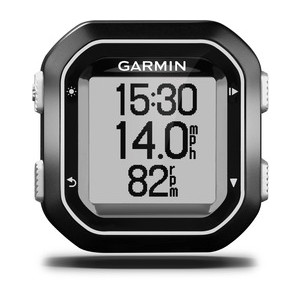
\includegraphics[width=11em]{figuras/cf-lg.jpg}}
    \label{fig:garmin}
\end{figure}
\centerline{Fonte: Página oficial do produto na Web\footnote{Disponível em:  <\url{https://buy.garmin.com/pt-BR/BR/cIntoSports-cCycling-p1.html}>. Acesso  em jun. 2015.}}

\section{Trabalhos científicos}
Entre os trabalhos científicos pesquisados estão as obras de Cesani e Dranka \citeyearpar{cesani2013} e Rosero \citeyearpar{gaidos2012}, ambos propuseram sistemas para auxiliar ciclistas em suas atividades. \par

Cesani e Dranka propuseram diretrizes para o desenvolvimento de uma aplicação \textit{mobile} com a intenção de auxiliar os ciclistas de Curitiba em seus trajetos. Para isso, eles estudaram o sistema de navegação GPS; as ciclovias e vias alternativas de Curitiba; o perfil do ciclista desta cidade; documentos sobre a infraestrutura urbana cicloviária e produtos relacionados usados pelos ciclistas de Curitiba. Como resultados, os autores definiram a fundamentação teórica da pesquisa e uma base para o desenvolvimento da interface homem-computador para um futuro protótipo funcional. \par

Rosero, em sua dissertação de mestrado, desenvolveu um protótipo para um sistema de treinamento e monitoramento para ciclistas (Figura \ref{fig:rosero}). Envolvendo a implementação de uma aplicação para plataforma Android e módulos de \textit{hardware} (tais como um módulo Bluetooth\footnote{Bluetooth é uma tecnologia de comunicação sem fio, baseada em ondas de rádio frequência de curto alcance. Possibilita comunicação eficiente e eficaz entre diferentes dispositivos eletrônicos \cite{gaidos2012}.}, sensores de frequência cardíaca, de percentual de oxigênio e de temperatura). Este sistema fornece informações dos sinais fisiológicos do usuário, processando e disponibilizando estas na rede social Twitter\footnote{\url{https://twitter.com}}, para que um treinador possa acompanhar os resultados.

\begin{figure}[t]
    \caption[Protótipo de \textit{hardware} desenvolvido por Rosero ligado ao capacete de um ciclista]{Protótipo de \textit{hardware} desenvolvido por Rosero ligado ao capacete de um ciclista \cite{gaidos2012}.}
    \centerline{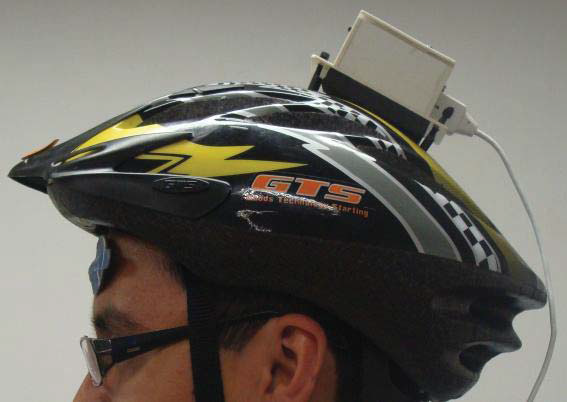
\includegraphics[width=18em]{figuras/rosero.png}}
    \label{fig:rosero}
\end{figure}

\section{Conclusões}
Neste capítulo foram apresentados trabalhos e sistemas existentes relacionados a temática e proposta do Pedal-to-Play. Um fator comum notável entre estes sistemas é que o público alvo são pessoas no geral já adeptas ao ciclismo, as quais o praticam por hábito e lazer ou como esporte. O projeto de Rosero foca no treinamento de ciclistas, usando um \textit{hardware} e \textit{software} personalizados para atender as necessidades destes e o trabalho de Cesani e Dranka é voltado para usuários que já utilizam a bicicleta como meio de locomoção em Curitiba. Nos aplicativos Strava e Runtastic, os usuários com maior visibilidade são aqueles que se dedicam integralmente ao esporte (o alto desempenho na atividade resulta em \textit{ranking} alto e vários \textit{badges}). O Pedal-to-Play por sua vez, ao se propor a trazer elementos de jogos à prática de ciclismo, foca também nas pessoas que têm mais familiaridade com \textit{video games} do que com o esporte (o exemplo clássico usado por Jane
McGonigal (\citeyearpar{mcgonigal2011reality}) sobre o quanto as pessoas têm se dedicado aos \textit{video games} é o do jogo \textit{online} \textit{World of
Warcraft}, ao somar todas as horas jogadas exclusivamente nele o resultado seria de 5,93 bilhões de anos, somente entre os anos de 2004 e 2011). O projeto visa  disponibilizar um ambiente cativante e motivador, também para este público não praticante envolver-se no ciclismo e torná-lo um hábito. No próximo capítulo será apresentado como a ideia do Pedal-to-Play foi projetada e desenvolvida.

% Metodologia
%Arquivo contendo o capítulo Metodologia
\chapter{Metodologia} \label{cap:metodologia}
A primeira etapa para o desenvolvimento do Pedal-to-Play será focada no levantamento de requisitos. Um dos requisitos já descrito nos objetivos deste trabalho é que este \textit{software} pretende ser multiplataforma e para garantir esta característica, pretende-se fazer uso das técnicas de desenvolvimento \textit{Web}. Segundo \citet{lopes2013}, o desenvolvimento \textit{Web} é democrático, aberto e acessível, pois praticamente, todo dispositivos \textit{mobile} possui um navegador (\textit{web browser}). Uma aplicação \textit{Web} garante acesso a um número maior de usuários do que uma aplicação nativa para um determinado dispositivo. Lopes também salienta que é cada vez mais comum usar as linguagens fundamentais da \textit{Web} para desenvolver aplicativos \textit{mobile}. \par

Demais requisitos envolverão: a definição dos \textit{frameworks} que serão utilizados; quais plataformas serão suportadas para execução da aplicação (sistemas operacionais \textit{mobile} e \textit{browsers}); a definição das ferramentas de desenvolvimento; as técnicas de gamificação a serem implementadas; as regras de negócio do sistema e os casos de uso. \par

Concluído o levantamento de requisitos, pretende-se iniciar a segunda etapa, a qual envolverá a prototipação da interface gráfica com o usuário (GUI\footnote{Acrônimo do inglês para \textit{Graphical User Interface}.}) e o desenvolvimento do \textit{template} do sistema. As interfaces terão como inspiração trabalhos e \textit{softwares} comerciais já existentes nessa categoria. O \textit{template} consistirá no desenvolvimento dos componentes comuns entre as telas da GUI, tais como a tela de \textit{login}, menu de navegação, cabeçalho, rodapé e tela de informações sobre o sistema. 

A terceira etapa do trabalho será focada na análise e modelagem do sistema. Envolverá o detalhamento dos casos de uso através de diagramas na linguagem UML (Unified Modeling Language\footnote{\url{http://www.uml.org/}}) para modelagem de sistemas. \par

A quarta etapa consistirá no desenvolvimento das funcionalidades do Pedal-to-Play e concomitantemente a dissertação da monografia e estudo das técnicas necessárias para implementação de cada funcionalidade. Pretende-se desenvolver as seguintes funcionalidades: \par

\begin{description}
\item[Rastreamento de Atividades] Envolve o uso dos recursos de \textit{hardware} dos dispositivo \textit{mobile} para captura de dados durante a prática da atividade de ciclismo. Pretende-se utilizar as funções do GPS\footnote{Acrônimo do inglês para \textit{Global Positioning System}.} para obter a distância do trajeto percorrido pelo usuário, possibilitando calcular a velocidade média e uma estimativa do total de calorias queimadas por ele.

\item[Módulo Avatar] Consiste nas funcionalidades do sistema responsáveis pela manutenção do avatar que representa virtualmente o usuário. Pretende-se desenvolver o avatar baseado em um conjunto de imagens bidimensionais, dividas em três categorias: o próprio avatar, os equipamentos dele e a bicicleta. Possibilitando ao usuário a customização de alguns atributos destas imagens (tais como cor e textura). A imagem \ref{fig:exavatar} é um exemplo ilustrativo da ideia do avatar a ser desenvolvido. 

\begin{figure}[h]
    \caption{Personagem da animação japonesa Yowamushi Pedal.}
    \centerline{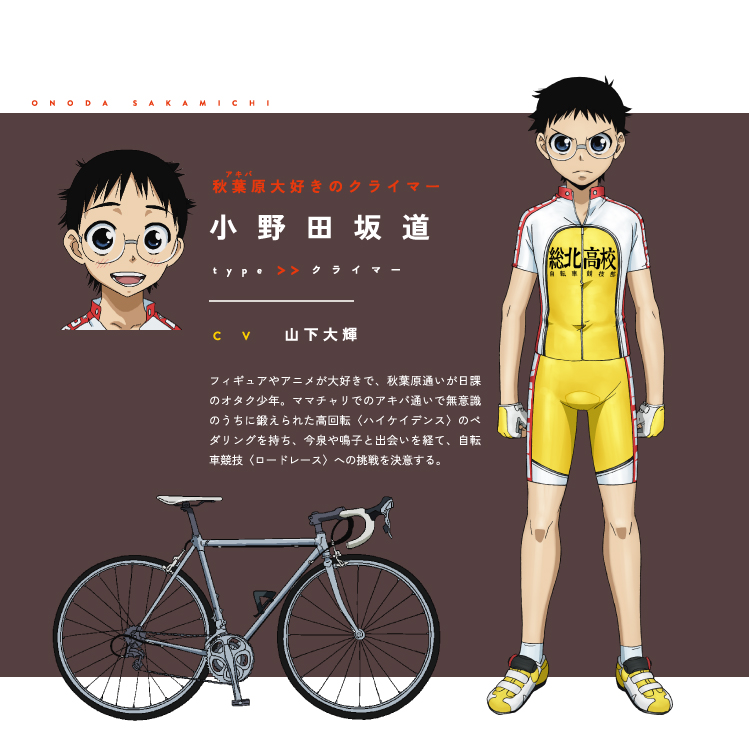
\includegraphics[width=20em]{figuras/exavatar.jpg}}
    \label{fig:exavatar}
\end{figure}
\centerline{Fonte: Página da \textit{Web} da qual a imagem foi retirada\footnote{Disponível em:  <\url{http://yowamushipedal.wikia.com/wiki/Onoda_Sakamichi}>. Acesso  em jul. 2015.}.}

\item[Lado do Servidor] O servidor consistirá na parte do sistema responsável pela persistência dos dados do usuário e a troca destes com a aplicação rodando no lado do cliente. \par

Atualmente o pódio das tecnologias para o desenvolvimento \textit{Web} do lado do Servidor está ocupado pelo PHP, em primeiro lugar; ASP.NET em segundo e o Java, em terceiro \cite{w3techs2015}. \par

Java \textit{Web} consiste na implementação das APIs de Servlets e JavaServer Pages (JSP). Servlet é a tecnologia usada pelo Java para geração de páginas HTML dinâmicas, são classes Java com HTML embutido. Páginas JSP consistem no inverso, são estruturadas como páginas HTML com código Java embutido. \par

ASP.NET é uma tecnologia da Microsoft, parte do .NET \textit{Framework} para desenvolvimento de aplicações \textit{Web}. As vantagens desta tecnologia envolvem a separação clara entre a interface do usuário e a lógica de programação; a familiaridade com o desenvolvimento \textit{desktop}; a ferramenta de desenvolvimento Visual Studio, com diversos recursos para facilitar o trabalho do desenvolvedor e a integração com todos os recursos do \textit{framework} .NET \cite{imar2014}. As desvantagens do ASP.NET são: sua limitação ao sistema operacional Windows e a licença de uso do Visual Studio não ser gratuita. \par

PHP é uma linguagem de programação presente em 10 milhões de sites no mundo inteiro. O PHP adiciona dinamismo às páginas estáticas e automatiza tarefas, diminuindo mão-de-obra. Possui portabilidade para várias plataformas \textit{desktop} (exemplos: Linux, Unix e Windows); possui código aberto e licença de uso gratuita; suporta vários bancos de dados (entre eles: MySQL, Oracle e PostgreSQL) \cite{niederauer2004, welling2003}. \par

Pretende-se usar a linguagem PHP para desenvolvimento do lado do servidor, pois comparado com as outras duas principais linguagens (ASP.NET e Java) o PHP se destaca por sua licença gratuita, portabilidade e suporte nativo (sem \textit{frameworks}) a funcionalidades que serão essenciais no software deste trabalho, tais como: gerenciamento de imagens, interpretação de arquivos JSON e acesso a banco de dados. \par

No quesito sistemas de gerenciamento de bando de dados (SGDB), os três mais usados atualmente segundo o \textit{site} da DB-Engines são o Oracle em primeiro lugar, o MySQL em segundo e o Microsoft SQL Server em terceiro. O MySQL possui licença de uso \textit{open source} e versão gratuita sem restrições, enquanto o Oracle e o Microsoft SQL Server são \textit{softwares} com licença de uso comercial, por estes motivos pretende-se fazer uso dele.

\item[Módulo Perfil do Usuário] Consiste no desenvolvimento da interface do perfil do usuário, contendo as principais informações dele, entre elas: nível, pontos, dados pessoais, avatar, \textit{ranking} e recompensas. Pretende-se que essa interface seja passível de customização.

\item[Módulo de Desafios] Envolve o mecanismo responsável pela geração de desafios, os quais consistem no cumprimento de certo objetivo proposto ao usuário. Pretende-se que os desafios sejam o meio para o usuário adquirir novos equipamentos, novas bicicletas, aumentar seu nível e \textit{ranking}, adquirir \textit{badges} e títulos.

\item[Integração com Redes Sociais] Envolve a implementação da funcionalidade que permite a integração com o Facebook, possibilitando ao usuário compartilhar seus dados, recompensas e aquisições nesta rede social. Esta funcionalidade é importante para divulgação do sistema e para propor engajamento social entre usuários do sistema e não usuários.
\end{description}

A etapa de conclusão deste trabalho será dedicada aos testes finais das funcionalidades desenvolvidas, à finalização da monografia e à defesa desta. \par 

Durante o decorrer deste trabalho serão estudados livros, trabalhos relacionados e tutoriais de uso das tecnologias necessárias para o  desenvolvimento do Pedal-to-Play. O material bibliográfico será pesquisado através de ferramentas de pesquisa eletrônica, como o Google Scholar e repositórios digitais, como o portal Lume, da Universidade Federal do Rio Grande do Sul. As palavras chave que direcionarão a pesquisa serão: \textit{mobile}, ciclismo, \textit{gamification}, \textit{web}, \textit{rastreamento de atividades} e geolocalização. Os tutorias serão buscados em plataformas de ensino digital, como o Mozilla Developer Network (MDN) e nos \textit{sites} oficiais de cada tecnologia. \par

Os produtos alvo deste trabalho serão o \textit{software} desenvolvido (gratuito e de código aberto) e a monografia, descrevendo o processo de pesquisa e desenvolvimento. \par


% Cronograma
%Arquivo contendo o capítulo Cronograma
\chapter{Cronograma} \label{cap:cronograma}
As atividades serão desenvolvidas conforme o cronograma mostrado na Tabela \ref{cronograma}.

\begin{table}[h]
\caption{Cronograma de atividades}
\begin{center}
\begin{tabular}{l|c|c|c|c}
\hline
\multirow{2}{*}{Tarefa} & 
\multicolumn{4}{c}{2015}\\& Ago & Set & Out & Nov 
    \\ \hline
    Levantamento de Requisitos  
        & x   & ~   & ~   & ~    
    \\ \hline
    Prototipação das Interfaces com Usuário
        & x   & ~   & ~   & ~  
    \\ \hline
    Desenvolvimento do \textit{Template} do Sistema
        & x   & ~   & ~   & ~      
    \\ \hline
    Análise do Sistema
        & x   & ~   & ~   & ~
    \\ \hline
    Desenvolvimento do Módulo de Rastreamento de Atividades 
        & ~   & x   & ~   & ~
    \\ \hline
    Desenvolvimento do Lado do Servidor                                 
        & ~   & x   & ~   & ~
    \\ \hline
    Desenvolvimento do Módulo Avatar                        
        & ~   & x   & ~   & ~
    \\ \hline
    Desenvolvimento Módulo Perfil do Usuário
        & ~   & ~   & x   & ~
    \\ \hline
    Desenvolvimento Módulo de Desafios
        & ~   & ~   & x  & ~
    \\ \hline
    Desenvolvimento da Integração com Redes Sociais         
        & ~   & ~   & x  & ~
    \\ \hline
    Finalização dos Testes                                     
        & ~   & ~   & ~  & x
    \\ \hline
    Finalização da Monografia                               
        & ~   & ~   & ~  & x
    \\ \hline
\end{tabular}
\end{center}
\label{cronograma}
\end{table}

% Conclusão
%\input{conclusão.tex}

% carrega o arquivo com as bibliografias e põe o capítulo com as referências neste lugar
\bibliography{bibliografia}

%% a partir daqui, todo capítulo novo é apêndice
%\appendix

%\chapter{Anexos e Apêndices}
%Destinam-se à inclusão de informações complementares ao trabalho, mas que não %são essenciais à sua compreensão. Os Apêndices devem apresentar material %desenvolvido pelo próprio autor, formatado de acordo com as normas. Já os %Anexos destinam-se à inclusão de material como cópias de artigos, manuais, %etc., que não necessariamente precisam estar em conformidade com o modelo, e %que não foram desenvolvidos pelo autor do trabalho.

%importa dicasLatexABNT.tex para o Apêndice 
%\chapter{Dicas de Latex e Normas ABNT}
Esta capítulo apresenta as coisas básicas que precisamos saber para fazer um TCC com Latex utilizando este modelo.

\section{O Básico do Latex}
Novo parágrafo pode ser feito por meio do comando par. \par
Outra forma é deixando uma linha em branco entre dois parágrafos.

Tudo o que está a direita de um \% é um comentário.
% Isto é um comentário
Para inserirmos o símbolo de porcento de forma proposital, precisamos colocar a barra invertida antes: 90\%.

Os caracteres \& \$ \# \% \_ \{ \} \^{} \~{} $\backslash$ são todos especiais e precisam ser escritos como comandos (com uma barra antes).
% tem um web app para ajudar a encontrar outros símbolos neste endereço: http://detexify.kirelabs.org/classify.html

Aspas são digitadas com duas crases no início e duas aspas simples no final: ``Texto entre aspas''

Estilos de fontes: \textbf{negrito}, \textit{itálico}, \textrm{romano}, \textsf{sans serif}, \texttt{maquina de escrever}, \textsc{caixa alta}.

Capítulos, seções e subseções são inseridas com:
\begin{verbatim}
\chapter{Um Capítulo} -> 1. Um Capítulo
\section{Uma Seção} -> 1.1 Uma Seção
\subsection{Uma Subseção} -> 1.1.1 Uma Subseção
\subsubsection{Uma Subsubseção} -> 1.1.1.1 Uma Subsubseção
\chapter*{Um Capítulo} -> Um Capítulo sem numeração
\end{verbatim}
Não se deve utilizar mais do que 4 níveis.

Ambientes são utilizados para definir uma região do texto que haverá tratamento especial:

\begin{verbatim}
O ambiente verbatin significa "ao pé da letra". 
Ex.: & $ # % _ { } ^ ~ $
\end{verbatim}

\begin{center}
O ambiente center escreve centralizado.
\end{center}

\begin{quote}
O ambiente quote é útil para fazer citações.
\end{quote}

Esta é a forma como se descreve itens:
\begin{description}
\item[Item 1] Isto significa uma coisa.
\item[Item 2] Este significa outra coisa.
\end{description}

Esta é a forma como se cita itens:
\begin{itemize}
\item Item 1;
\item Item 2.
\end{itemize}

E esta é a forma como se enumera itens:
\begin{enumerate}
	\item Qual a alternativa correta?
		\begin{enumerate}
			\item esta.
			\item ou esta.
		\end{enumerate}
\end{enumerate}

Fórmulas matemáticas são colocadas dentro de um ambiente matemático. Tudo neste ambiente é considerado elemento numérico e possui uma formatação diferente. Os comandos aceitos também podem mudar.

Equações matemáticas em destaque são inseridas da seguinte maneira:

% tem um web app para ajudar a fazer equações neste endereço: http://mathurl.com/
% ou aqui: http://webdemo.visionobjects.com/#/demo/equation
$$
x=\frac{-b\pm\sqrt{b^2-4ac}}{2a}.
$$

ou 

\begin{equation}
\begin{array}{rcl}
x_2 - x_1 &\geq& b_1 r_1\\
x_2 - x_1 &\geq& b_2 r_2\\
x_2 - x_1 &\geq& b_n r_m\\
b_1 + b_2 + ... + b_n &=& 1
\end{array}
\end{equation}

enquanto equações inline são feitas desta forma: $r_i (1\leq i \leq m)$.

\section{Convenções}
Escreva o título e os capítulos, seções, subseções, etc. sempre com a primeira letra de cada palavra importante em Maiúsculo e o restante em minúsculo. O Latex se encarregará de deixar tudo MAIÚSCULO onde for necessário.

Nenhuma seção deve ficar sem texto.

Utilize siglas para não ter de repetir muitas vezes o mesmo texto. Neste caso, na primeira ocorrência coloque o significado antes e a sigla entre parênteses (aproveitando também para adiciona-la à lista de siglas). Nas demais ocorrências, apenas coloque a sigla. 
Ex.: ...execução do algoritmo de  \textit{Threshold Accepting} (TA) sobre um circuito. A versão do algoritmo de TA utilizada...

Palavras em \textit{English} ou outra lingua estrangeira devem estar em itálico. Utilize \textbf{negrito} quando for necessário destacar alguma coisa.

\section{Figuras e Tabelas}

Todas as figuras e tabelas devem estar referenciadas no texto e com a descrição acima delas. Não são permitidos outros nomes tais como: quadro, imagem, etc.  Comece a descrição com letra maiúscula e faça o restante em minúscula (exceto siglas), terminando com um ponto final.

Se buscada em alguma obra publicada, a citação deve sempre aparecer. Pode ser colocada entre parênteses, como no exemplo da Figura \ref{fig:dsp2}, ou preferencialmente abaixo após a palavra "Fonte: ", como no exemplo da Tabela \ref{tab:comp1}. Observando que na LISTA DE FIGURAS/TABELAS a fonte/citação não deve aparecer.

É possível colocar as figuras de lado e também redimensiona-las através dos parâmetrosdo Latex, como nos exemplos das Figuras \ref{fig:dsp} e \ref{fig:dsp2}. Dê preferência por imagens vetoriais ou em PDF, para não perder qualidade. Procure deixar os textos das figuras com o mesmo tamanho das letras no restante do documento.

\begin{figure} % [h] -> utilize este parâmetro para forçar nesta posição
    \caption{Segundo a ABNT, a descrição deve ficar acima da figura}
    \centerline{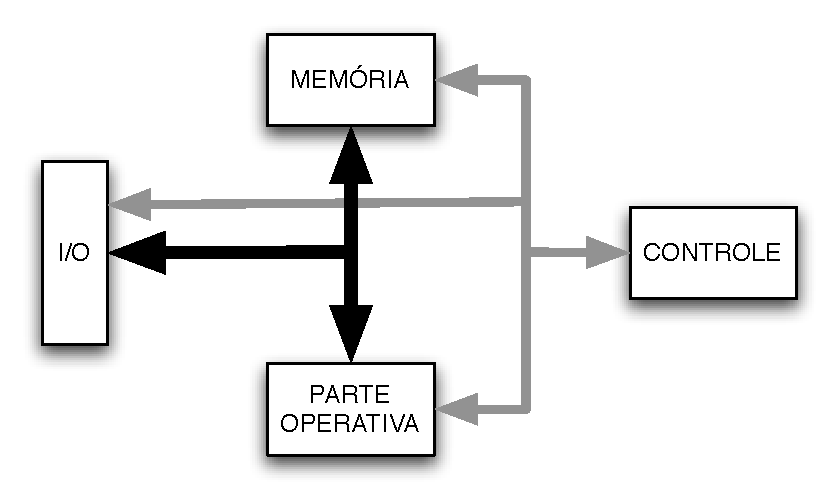
\includegraphics[width=20em]{figuras/dsp}}
    \label{fig:dsp}
\end{figure}

\begin{sidewaysfigure}
    % entre colchetes a descrição que vai para a lista de figuras, sem legenda (opcional)
    \caption[Descrição com citação]{Descrição com citação \cite{artigo}}
    \centerline{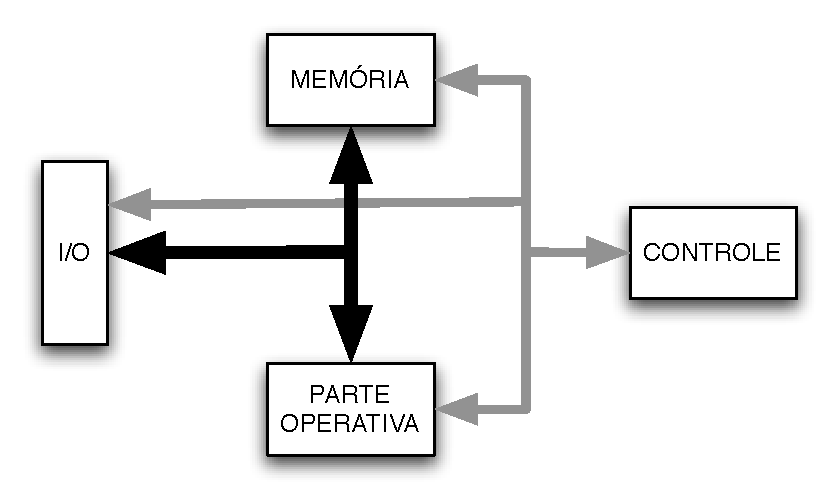
\includegraphics[width=40em]{figuras/dsp}}
    \label{fig:dsp2}
\end{sidewaysfigure}

As tabelas devem ser ``abertas'' dos lados (sem as linhas laterais), como no exemplo da Tabela \ref{tab:comp1}, isto torna a imagem mais limpa e clara.

% tem um web app para ajudar a fazer tabelas no latex neste endereço: http://truben.no/latex/table/
\begin{table}
    \centering
    \scalefont{0.93} %necessário eventualmente para reduzir o tamanho da tabela
    \caption{Comparação entre X e Y.}
    \begin{tabular}{c|c|c|c|c|c} \hline
        \multirow{2}{*}{\bf{Célula}} & \multirow{2}{*}{\# \bf{Trans.}} & \multicolumn{3}{|c|}{\bf{Largura} ($\mu m$)} & \bf{Tempo Exec. (s)}\\ \cline{3-6} 
         &  & Std. Cell & ASTRAN & \% & ASTRAN \\ \hline \hline
        AND2X4& 6 & 1 & 1,2 & 20 & 10 \\ \hline
        FAD1X4& 28 & 3,6 & 4 & 12 & 750\\ \hline
        FAD1X9& 28 & 4,2 & 4,2 & 0 & 1800\\ \hline
        HAD1X9& 14 & 2,4 & 2,4 & 0 & 30\\ \hline
        HAD1X18& 18 & 2,8 & 2,8 & 0 & 205\\ \hline
        INVX0 & 2 & 0,6 & 0,6 & 0 & 1\\ \hline
        TOTAL& - & 28 & 29 & 3,6 &-\\ \hline
    \end{tabular}
    {\\ Fonte: \cite{artigo}.}
    \label{tab:comp1}
\end{table}

\section{Citações}
Há duas formas de se fazer uma citação: a citação indireta ou livre e a citação direta ou textual. Todas as citações devem trazer a identificação de sua autoria.

No Latex, inserimos citações utilizando o formato bibtex. Para tanto, precisamos catastrar os dados da citação no arquivo .bib e em seguida citarmos no .tex com o comando cite. Colocar preferencialmente em ordem cronológica, com o mais recente por último \cite{livro, artigo, tese, capitulo, paper, site, apresentacao}.

\subsection{Citação Indireta}
Aquela citação na qual expressamos o pensamento de outra pessoa com nossas próprias palavras. Ex.:

Segundo o trabalho de Silva e Santos \citeyearpar{artigo}, o céu é azul porque...

O céu é azul porque... \cite{artigo}.

\subsection{Citação Direta}
São aquelas em que se transcreve exatamente as palavras do autor citado. As citações diretas ou textuais podem ser breves ou longas. São consideradas breves aquelas cuja extensão não ultrapassa três linhas e devem vir entre aspas. As citações com mais de três linhas são chamadas de longas (sem aspas) e devem receber um destaque especial com recuo.  Ex.:

Segundo Fulano, ``Quando a luz passa através de um prisma, seu espectro é dividido em sete cores monocromáticas'' \citeyearpar{artigo}.

\begin{quote}
Quando a luz passa através de um prisma, seu espectro é dividido em sete cores monocromáticas, eis que surge um arco-íris de cores. A atmosfera faz o mesmo papel do prisma, atuando onde os raios solares colidem com as moléculas de ar, água e poeira e são responsáveis pela dispersão do comprimento de onda azul da luz. \cite{artigo}
\end{quote}

Havendo supressão de trechos dentro do texto citado, faz-se a indicação com reticências entre colchetes [...]. De forma similar, para interpelação, acréscimo ou comentário durante a citação, deve-se fazê-lo também entre colchetes. No início ou no fim da citação, as reticências são usadas apenas quando o trecho citado não é uma sentença completa.Ex.:

``Também chamado de corpo do trabalho, [o desenvolvimento] tem por finalidade expor [...] a explicitação do assunto a ser abordado...'' \cite{artigo}.

\section{Notas de Rodapé}
As notas de rodapé\footnote{Nota sobre a palavra rodapé} são usadas nos documentos impressos para explicar ou fazer comentários detalhados.


\end{document}
